\tightsection{Quality Improvement via Prediction}
\label{sec:improvement}

Previous sections have established our prediction algorithm can achieve near-optimal accuracy. In this section, we empirically study the impact of prediction accuracy on video quality improvement, i.e., does a good prediction lead to high improvement. It should be noticed that the possible improvement is bounded by the actual difference between the performance of resources (e.g., CDN or bitrate). As pointed out in \Section~\ref{sec:intro}, current industrial practice however, only allows coarse grain decisions (e.g., CDN-level rather than server-level) and the different at such level is much less significant than finer-grain ones. Therefore, though based on our dataset our quantitative results do not show remarkable improvement under CDN or bitrate selection, we expect to see higher improvement with more fine-grain selection enabled and thus larger room of improvement.

Specifically, we aim to answer two questions:
\begin{packedenumerate}
	\item How does prediction accuracy impact quality improvement?
	\item How does quality diversity among multiple decisions impact quality improvement? \xil{a bit vague}\jc{Xi, please write a better one.}
\end{packedenumerate}

\tightsubsection{Methodology}
We study these questions by using offline analysis methodologies including trace-driven analysis. As we will introduce in next sections, we have built GO system that runs in real world, and we use A/B testing  to demonstrate GO's behavior and its quality improvement in the wild in \Section~\ref{sec:eval}. However, we believe these questions should be better addressed using offline trace-driven analysis because the real world experiments has four limitations.
\begin{packedenumerate}
	\item Limited coverage: As we will explain, the real world experiments only have access to the video traffic of one video site on one type of OS. The stricts its coverage of classes of traffic in both video genres and streaming protocol.
	\item Limited scale of simultaneous expriments: Since we only control one site's traffic in real world experiments, it is not feasible to compare many configurations or algorithms in parallel (empirically, at most 3-4) and ensure each of them receive sufficient traffic to draw confident conclusions.
	\item Limited diversity in performance: As we will see, the improvement in quality is greatly impacted by the diversity and variability of the performance outcome of different decisions (e.g., different CDNs). However, we can only observe a small number of possible patterns in performance diversity.
	\item Limited controlled experiments: Finally, it is impossible to conduct sensitivity analysis (as in this section) where we would like to see the impact of changing one parameter (e.g., CDN performance) at a time with controlled amount.
\end{packedenumerate}


This section uses three input to answer the two high-level questions. We now describe them in the order of closeness to realism and in reverse order of degree of controllability.

\myparatight{Counterfactual input} This approach is the closest to real-world A/B testing. The basic idea is that we first collect a dataset in which the decisions are randomly made for each client (called {\it random dataset}) and collect the quality metrics of each video session. Then we evaluate a given decision algorithm by picking the sessions for which the decision the algorithm makes matches the decisions in the random dataset. In \Section~\ref{sec:counterfactualtesting}, we show that this approach is unbiased. 
By using this methodology, we are able to replay multiple algorithms on the data sets.

\myparatight{Augmented trace-driven input} While counterfactual input is useful in evaluating different algorithms, we cannot use it to estimate the ``would-be" performance of an ``oracle" approach (e.g., how the performance would be if another decision were taken), which requires data extrapolation. In addition, counterfactual input only has one site traffic and only provide limited coverage. To remedy these limitations, we generate an augmented trace-driven synthetic dataset in which we extrapolate for each session the ``true'' quality outcome of all its possible decisions. The basic idea of this extrapolation  is that for each session $s$, its outcome of each decision $d$ is drawn from the distribution of outcomes of this decision $d$ on other sessions exactly matching the same attributes with $s$. Having ensured that quality outcomes in the synthetic scenario are known for any decision, it is possible to identify an {\it oracle} approach that always makes the best decision. However, the evaluation is could be biased by the extrapolation.

\myparatight{Controlled synthetic input} Both previous methodology lacks control, i.e., if no major outage or other events happen in the data set, we cannot evaluate GO performance under those scenarios. Thus we also use fully controlleable input in which the true outcomes (i.e., ``ground truth'') of each decision is controlled.





\tightsubsection{Behavioral study}
We first explain the GO's prediction-based decision making and use controlled synthetic input to confirm its behavior -- GO identifies the performance changes and switches decision accordingly if needed.

\myparatight{Prediction-based dececision making} GO's decision algorithm simply selects for each session under prediction the decision that has the best predicted quality in a predetermined metric (e.g., buffering ratio). Note that GO always leaves a small fraction of traffic to be randomly allocated to guarantee that each decision will have at least certain fraction of traffic even when that decision is not the best.


\begin{figure}[h!]
\centering
 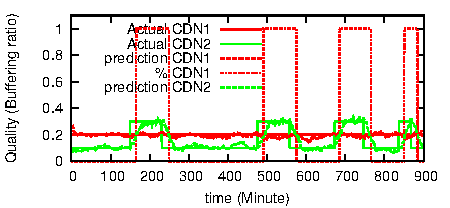
\includegraphics[width=0.5\textwidth] {figures/behavior-evaluation/simple-change.pdf}
\tightcaption{Case for behavioral study}
\label{fig:behavioral}
\end{figure}

\myparatight{Case study} We simulate a scenario in which a sudden change in performance of one group causes GO to switch decision accordingly. Figure~\ref{fig:behavioral} shows the behavior of sessions in one ASN when provided with two CDNs to choose from. We only controll buffering ratio as quality metric. The mean of buffering ratio of CDN1 is stably at 0.2 and that of CDN2 changes between 0.1 and 0.25, with a random interval. Each quality sample of a CDN is generated so that its buffering ratio has a Guassian noise with standard deviation of 0.01 from mean. This figure shows clearly that under this configuration, GO is able to switch to the best CDN accordingly with an expected delay (as it uses a 30-minute sliding window). Note that there is always a small amount of randomized traffic, so the change on each decision can be detected. %As a side-effect, it takes longer for GO to detect that CDN2 has bad bad quality than when it has good quality, because the number of samples from CDN2 when it has bad quality (only randomized traffic) is smaller than when it has good quality (all traffic).

%\xil{are we going to do something about that point or ack it is an issue.}

\tightsubsection{Impact of prediction accuracy}

To quantify the impact of prediction accuracy, we need to generate prediction with certain prediction error and see the improvement. To do this, we use both counterfactual input and augmented trace-driven input. 

\myparatight{Counterfactual testing}
In counterfactual input, we use GO to do prediction and add noise of varying magnitude to the prediction result. The additional noise follows a Gaussian random with increasing standard deviation.
This allows us to see how much worse the quality improvement will be if we have more noise in prediction result. 

\begin{figure}[h!]
\centering
 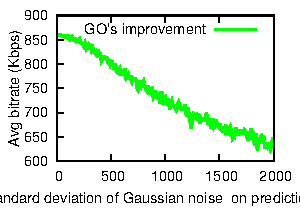
\includegraphics[width=0.35\textwidth] {figures/newfig/trendNoise-metricId1-keyGlobal-partition.pdf}
\tightcaption{Impact of the additional noise to prediction on quality improvement.}
\label{fig:trace-accuracy-1}
\end{figure}

Figure~\ref{fig:trace-accuracy-1} shows the GO improvement from a baseline random algorithm which selects a uniformly random decision. The figure shows an near linear degredation on improvement in average bitrate -- average bitrate improvement reduces 50Kbps with Gaussian noise increases 200Kbps in its standard deviation.



\myparatight{Augmented trace-driven testing}
Although counterfactual testing provides unbiased evaluation on the impact prediction noise, it does not allow us to control the prediction error because the true outcome is not available. In this part, we use the augmented trace-driven testing to quantify the impact of prediction error on quality improvement. Given a session and one decision, if the true quality is $q$ and $p$ is the prediction made by GO, we use a parameter called stretch $r$ to change the prediction $p$ to new prediction $p'=q+(p-q)r$ such that the prediction error is exactly stretched by $r$. 
Moreover, we could compare with an oracle which always makes the decision with the best quality. To simplify the discussion, we assume each session has two  possible decisions. 

\begin{figure}[h!]
\centering
 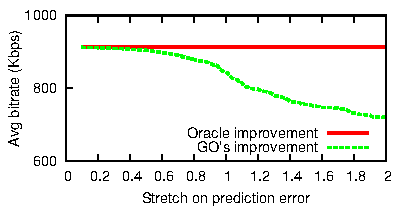
\includegraphics[width=0.35\textwidth] {figures/newfig/trendAccuracy-metricId1-keyGlobal-partition.pdf}
\tightcaption{Impact of GO prediction accuracy with varying stretch rate on quality improvement.}
\label{fig:trace-accuracy-2}
\end{figure}

Figure~\ref{fig:trace-accuracy-2} shows the results with average bitrate as the quality metric. We consider a baseline algorithm which select a uniformly random decision. The top line is the improvement of oracle approach from the baseline algorithm, which should be static. The bottom line shows the improvement of GO from the basline algorithm. 
It shows a clear degredation in improvement and such degradation is linear from stretch ratio of 0.9 -- after this point, with prediction error raised by every 10\%, the improvement in average bitrate decreases by 20Kbps. It suggests that the improvement is sensitive to accuracy if GO's prediction becomes worse. Also, note that with larger stretch rate, the improvement stablizes.

\xil{conclusion seems a bit weak}



\tightsubsection{Impact of quality diversity}

To quantify the impact of quality diversity among multiple decisions, we fix the prediction accuracy provided by GO. Intuitively, it is expected that with increasing diversity among multiple decisions, we should see that GO's performance should be close to the oracle approach since the gap between decisions' outcome is so large that the best decision will be made with any prediction error. 

To confirm this intuition, we use a stretch parameter $r$ to control the quality diversity between multiple decisions. To simplify the discussion, we assume each session has two possible decisions. Given a session with the true quality of two decisions being $q_1, q_2$ (assume $q_1\leq q_2$), we change their value to $q_1'=q_1, q_2=q_1+(q_2-q_1)r$. We again use two improvement from baseline and room of improvement to characterize the quality improvement.

\begin{figure}[h!]
\centering
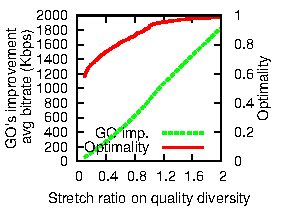
\includegraphics[width=0.35\textwidth] {figures/newfig/trendDiversity-metricId1-keyGlobal-partition.pdf}
\tightcaption{Impact of quality diversity on quality improvement.}
\label{fig:trace-diversity}
\end{figure}

Figure~\ref{fig:trace-diversity} shows the result with average bitrate as the quality metric. The left y axis shows the improvement of GO based on the random baseline algorithm. It shows close to linear increase with more quality diversity between decisions. 
The right y axis shows the room of improvement which is the difference between GO's improvement and oracle's improvement. With close-to-zero stretch parameter, the room of improvement reduces to zero simply because even the oracle approach cannot make much benefit from selecting the best decision as the gap is minimized. 
In the middle of the figure, it shows a close to linear relationship between stretch on quality diversity and room of improvement, with quality diversity increases by every 10\%, the room of improvement decreases by 20Kbps. 



\tightsubsection{Summary of observations}
\begin{packedenumerate}
	\item Under controlled experiments, GO identifies performance change and switches decisions accordingly.
	\item Quality improvement is linear to prediction error -- 10\% reduction in prediction error yields to 20Kbps in quality improvement.
	\item GO's quality improvement increases linearly with quality diversity between decisions and such improvement becomes closer-to-optimal with larger quality diversity.
\end{packedenumerate}

\xil{overall i feel the figures and conclusions from this section is not very concrete. there should be quantitative conclusions.}





































